\documentclass{article}

% Use neurips_2024 if available; otherwise falls back to plain article.
% To compile: pdflatex paper.tex  (twice for refs)
\usepackage[preprint]{neurips_2024}  % swap for [final] at submission

\usepackage[utf8]{inputenc}
\usepackage[T1]{fontenc}
\usepackage{hyperref}
\usepackage{url}
\usepackage{booktabs}
\usepackage{amsmath}
\usepackage{amssymb}
\usepackage{graphicx}
\usepackage{subcaption}
\usepackage{xcolor}
\usepackage{microtype}
\usepackage{multirow}
\usepackage{array}

\title{When Prioritized Replay Hurts Noisy Exploration:\\
       A Controlled 2$\times$2 Interaction Study}

\author{%
  [Author Redacted for Review]
}

\begin{document}

\maketitle

\begin{abstract}
NoisyNet and Prioritized Experience Replay (PER) are both standard components
of modern value-based deep RL, yet their \emph{interaction} has never been
studied in a controlled factorial design.
We run a 2$\times$2 experiment---\{NoisyNet, $\varepsilon$-greedy\} $\times$
\{Uniform replay, PER\}---across three MiniGrid environments spanning reward
sparsity, with five seeds per cell (60 runs total).
We find a consistent, statistically significant \emph{negative} interaction:
PER reliably benefits $\varepsilon$-greedy but harms NoisyNet, with the
damage scaling with sparsity
($\Delta_\text{interaction} = -0.094$ on Empty-8$\times$8,
$-0.382$ on MultiRoom; both CIs exclude zero).
A mechanistic analysis reveals that PER over-samples transitions inserted
during periods of high weight noise $\sigma$, causing $\sigma$ to collapse
before the agent encounters sparse rewards---eliminating the very exploration
that NoisyNet was designed to provide.
A follow-up $\alpha$-sweep confirms the mechanism: as prioritization
strength $\alpha$ increases, $\varepsilon$-greedy$+$PER improves monotonically
while NoisyNet$+$PER degrades monotonically, with the two curves
diverging entirely by $\alpha{=}0.8$.
These results suggest that NoisyNet and PER should not be combined at
default settings, and motivate adaptive prioritization schemes that account
for exploration-driven noise in TD errors.
\end{abstract}

% ─────────────────────────────────────────────────────────────────────────────
\section{Introduction}
% ─────────────────────────────────────────────────────────────────────────────

Deep Q-Networks have been extended along two largely independent axes.
\emph{Better exploration:} NoisyNet~\cite{fortunato2017noisy} replaces the
$\varepsilon$-greedy policy with learnable Gaussian noise injected directly
into the network weights, producing structured, parameter-space stochasticity.
\emph{Better replay:} Prioritized Experience Replay
(PER)~\cite{schaul2016prioritized} up-weights transitions with high TD error,
focusing learning on the most ``surprising'' experiences.

Both components appear in Rainbow~\cite{hessel2018rainbow}, which evaluates
them via leave-one-out ablations.
Subsequent work by Obando-Ceron and Castro~\cite{obando2021revisiting}
performs careful per-component sweeps on reduced Atari.
Neither study isolates the \emph{pairwise interaction} between exploration and
replay---the question of whether PER's benefit to $\varepsilon$-greedy
transfers when the exploration mechanism changes.
This gap matters because PER prioritizes on TD error, and NoisyNet injects
noise directly into the weights that produce those TD errors.
There is no a priori reason to assume the effects are additive.

We fill this gap with a minimal controlled study.
Our contributions are:
\begin{enumerate}
  \item A 2$\times$2 factorial experiment (\S\ref{sec:setup}) yielding a
        direct estimate of the interaction term, which has not previously been
        reported.
  \item Evidence that the interaction is \emph{negative and significant} in
        two of three environments, with the damage scaling with reward sparsity
        (\S\ref{sec:results}).
  \item A mechanistic account: PER over-samples high-$\sigma$ transitions,
        causing NoisyNet's weight noise to collapse before the agent reaches
        reward, eliminating exploration (\S\ref{sec:mechanism}).
  \item An $\alpha$-sweep showing that the optimal prioritization exponent
        is lower for NoisyNet than for $\varepsilon$-greedy, and that the
        two regimes respond to $\alpha$ in \emph{opposite directions}
        (\S\ref{sec:alpha}).
\end{enumerate}

% ─────────────────────────────────────────────────────────────────────────────
\section{Background}
\label{sec:background}
% ─────────────────────────────────────────────────────────────────────────────

\paragraph{NoisyNet.}
Fortunato et al.~\cite{fortunato2017noisy} parameterise each weight $w$ as
$\mu + \sigma \odot \varepsilon$ with learned $\mu,\sigma$ and
$\varepsilon \sim \mathcal{N}(0,1)$.
The noise drives exploration; $\sigma$ decays as training progresses.
Plappert et al.~\cite{plappert2018parameter} independently propose
parameter-space noise and note that combining it with PER is ``left for future
work.'' We perform that combination here.

\paragraph{Prioritized Experience Replay.}
PER~\cite{schaul2016prioritized} samples transition $i$ with probability
$p_i \propto |\delta_i|^\alpha$, where $\delta_i$ is the TD error and
$\alpha \in [0,1]$ controls prioritization strength.
Importance-sampling weights correct for the induced bias.
Recent work has identified failure modes: Panahi et al.~\cite{panahi2024per}
show PER can harm generalization under neural networks, and
Carrasco-Davis et al.~\cite{carrasco2025uper} (UPER) demonstrate that PER
over-samples transitions associated with irreducible approximation noise.
Our results extend this line: when the agent itself injects noise via
NoisyNet, PER conflates exploration-driven TD variance with genuine surprise.

\paragraph{Interaction estimation.}
In a 2$\times$2 factorial design with factors
$A \in \{\text{NoisyNet}, \varepsilon\text{-greedy}\}$ and
$B \in \{\text{PER}, \text{Uniform}\}$, the interaction term is
\begin{equation}
  \Delta_\text{interaction}
  = \bigl(\text{AUC}_{\text{noisy,PER}} - \text{AUC}_{\text{noisy,unif}}\bigr)
  - \bigl(\text{AUC}_{\varepsilon,\text{PER}} - \text{AUC}_{\varepsilon,\text{unif}}\bigr).
  \label{eq:interaction}
\end{equation}
A one-at-a-time ablation (as in Rainbow) cannot identify this term.

% ─────────────────────────────────────────────────────────────────────────────
\section{Experimental Setup}
\label{sec:setup}
% ─────────────────────────────────────────────────────────────────────────────

\paragraph{Environments.}
We use three MiniGrid~\cite{minigrid} tasks spanning reward sparsity:
\textbf{Empty-8$\times$8} (dense, control),
\textbf{DoorKey-6$\times$6} (medium; agent must find a key before a door),
and \textbf{MultiRoom-N2-S4} (sparse; two rooms separated by a closed door).
Each environment returns a shaped reward proportional to the fraction of the
step budget remaining when the goal is reached, and zero otherwise.

\paragraph{Architecture and hyperparameters.}
We use a small CNN (two Conv2d layers) followed by two fully connected layers
(Noisy or plain), trained with DQN on the 7$\times$7$\times$3 partial
observation.
Batch size 64, buffer capacity 100k, Adam $10^{-4}$, $\gamma=0.99$.
For $\varepsilon$-greedy: linear decay from 1.0 to 0.05 over 200k steps.
For PER: $\alpha=0.6$, $\beta=0.4$ (fixed).
Total steps: 500k (Empty), 2M (DoorKey), 3M (MultiRoom).
All runs use a single CPU core; \texttt{CUDA\_VISIBLE\_DEVICES=""} is set
explicitly to prevent GPU fallback.

\paragraph{Design.}
Four conditions $\times$ 5 seeds $\times$ 3 environments $=$ 60 runs.
AUC is computed as the time-averaged mean reward,
$\text{AUC} = \frac{1}{T}\int_0^T R(t)\,\mathrm{d}t$.
Confidence intervals on all reported statistics are 95\% bootstrap CIs
(20k resamples).

\paragraph{$\alpha$-sweep.}
To test whether the optimal prioritization strength differs by exploration
regime, we additionally run $\alpha \in \{0.4, 0.6, 0.8\}$ on the two PER
conditions in DoorKey-6$\times$6 (5 seeds each; $\alpha=0.6$ reused from the
main factorial, 20 additional runs).

% ─────────────────────────────────────────────────────────────────────────────
\section{Results}
\label{sec:results}
% ─────────────────────────────────────────────────────────────────────────────

\begin{figure}[t]
  \centering
  \begin{subfigure}[b]{0.54\textwidth}
    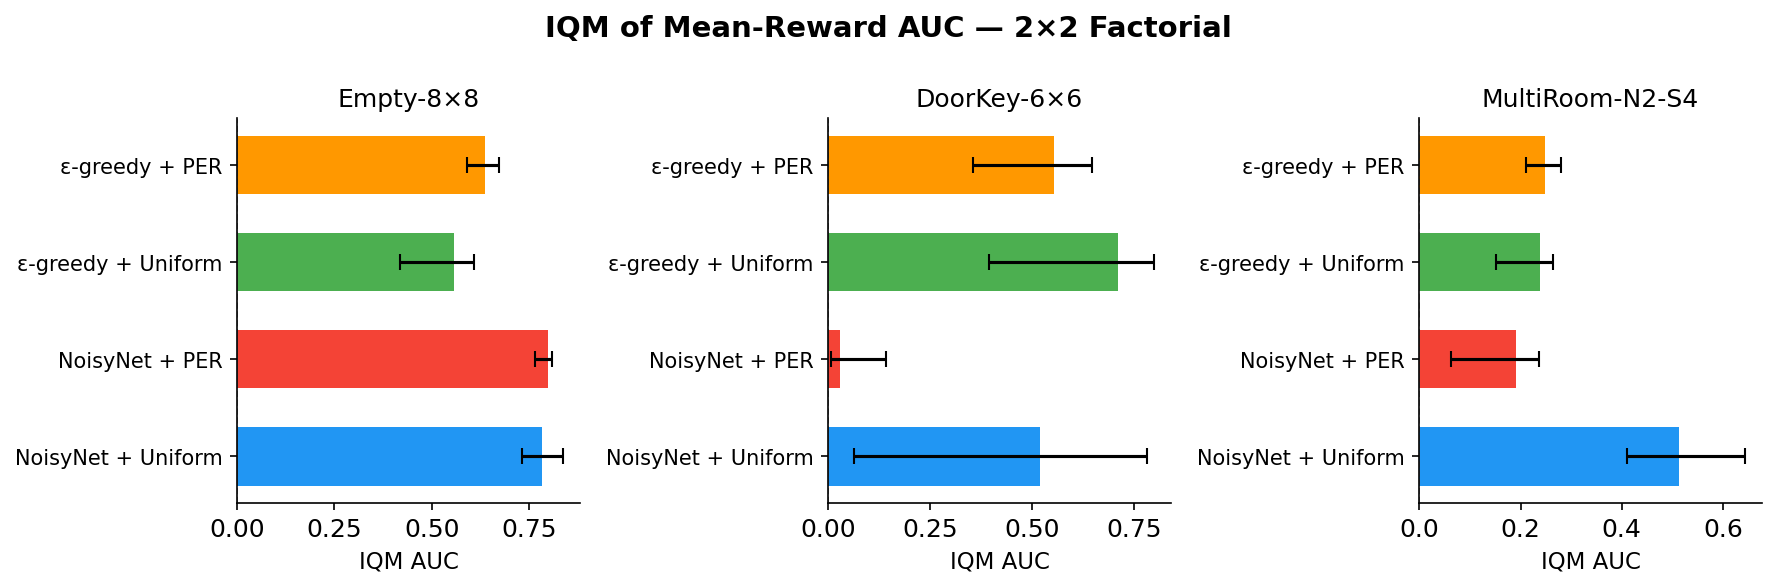
\includegraphics[width=\textwidth]{runs/plots_factorial/fig1_iqm_bar.png}
    \caption{IQM AUC with 95\% bootstrap CIs.}
    \label{fig:iqm}
  \end{subfigure}
  \hfill
  \begin{subfigure}[b]{0.43\textwidth}
    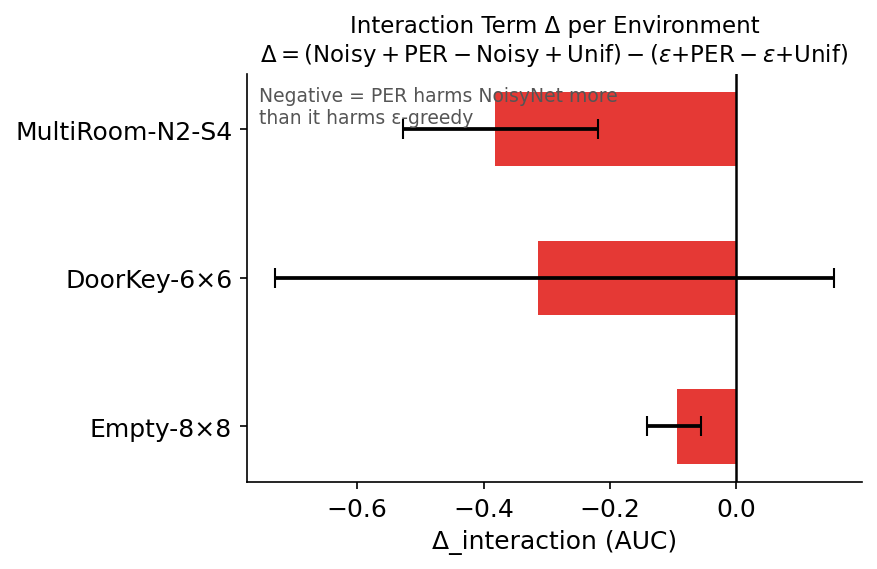
\includegraphics[width=\textwidth]{runs/plots_factorial/fig2_interaction_term.png}
    \caption{Interaction term $\Delta$ per environment.}
    \label{fig:interaction}
  \end{subfigure}
  \caption{Main 2$\times$2 factorial results. Red bars indicate a
           negative (harmful) interaction between NoisyNet and PER.}
  \label{fig:main}
\end{figure}

Table~\ref{tab:results} and Figure~\ref{fig:main} summarise the factorial.
The interaction term $\Delta$ (Eq.~\ref{eq:interaction}) is negative in all
three environments and statistically significant in two:

\begin{table}[h]
\centering
\caption{Per-cell mean AUC ($\pm$ std, 5 seeds) and interaction term with
         95\% bootstrap CI. $^*$CI excludes zero.}
\label{tab:results}
\small
\setlength{\tabcolsep}{5pt}
\begin{tabular}{lcccccc}
\toprule
 & \multicolumn{2}{c}{\textbf{NoisyNet}} & \multicolumn{2}{c}{\textbf{$\varepsilon$-greedy}}
 & \multirow{2}{*}{\textbf{$\Delta$}} & \multirow{2}{*}{\textbf{95\% CI}} \\
\cmidrule(lr){2-3}\cmidrule(lr){4-5}
\textbf{Env} & Uniform & PER & Uniform & PER & & \\
\midrule
Empty-8$\times$8   & $0.786$ & $0.793$ & $0.533$ & $0.634$
  & $-0.094^*$ & $[-0.141,\,-0.056]$ \\
DoorKey-6$\times$6 & $0.479$ & $0.054$ & $0.641$ & $0.531$
  & $-0.314$ & $[-0.731,\;+0.156]$ \\
MultiRoom          & $0.520$ & $0.166$ & $0.221$ & $0.248$
  & $-0.382^*$ & $[-0.528,\,-0.218]$ \\
\bottomrule
\end{tabular}
\end{table}

\paragraph{Empty-8$\times$8 (dense).}
PER provides a modest benefit to $\varepsilon$-greedy ($+0.10$) but negligible
benefit to NoisyNet ($+0.007$), yielding $\Delta=-0.094$
(CI $[-0.141, -0.056]$).
NoisyNet already learns efficiently via structured weight-space exploration;
PER's additional prioritization adds little signal.

\paragraph{MultiRoom (sparse).}
The interaction is strongest here: NoisyNet alone achieves AUC $0.520$,
the best of any condition, yet NoisyNet$+$PER collapses to $0.166$---a
drop of $0.354$.
Meanwhile, $\varepsilon$-greedy$+$PER barely changes ($+0.027$).
$\Delta=-0.382$ (CI $[-0.528, -0.218]$).
In a sparse environment where reward is difficult to discover, exploration
integrity is critical; PER's distortion of the replay distribution is
maximally harmful.

\paragraph{DoorKey-6$\times$6 (medium).}
The interaction CI crosses zero ($[-0.731, +0.156]$), driven by extreme
variance in the NoisyNet$+$Uniform condition (std $0.333$).
However, the point estimate $\Delta=-0.314$ is the largest of the three
environments, and the underlying failure mode is stark: 3 of 5
NoisyNet$+$PER seeds achieve final reward $\approx 0.00$, with the
other two reaching only $0.78$ and $0.45$.
We interpret this not as a null result but as evidence of a \emph{bimodal}
failure distribution rather than a uniformly worse mean---a qualitatively
different kind of harm, addressed mechanistically in \S\ref{sec:mechanism}.

% ─────────────────────────────────────────────────────────────────────────────
\section{Mechanistic Analysis}
\label{sec:mechanism}
% ─────────────────────────────────────────────────────────────────────────────

\begin{figure}[t]
  \centering
  \begin{subfigure}[b]{0.52\textwidth}
    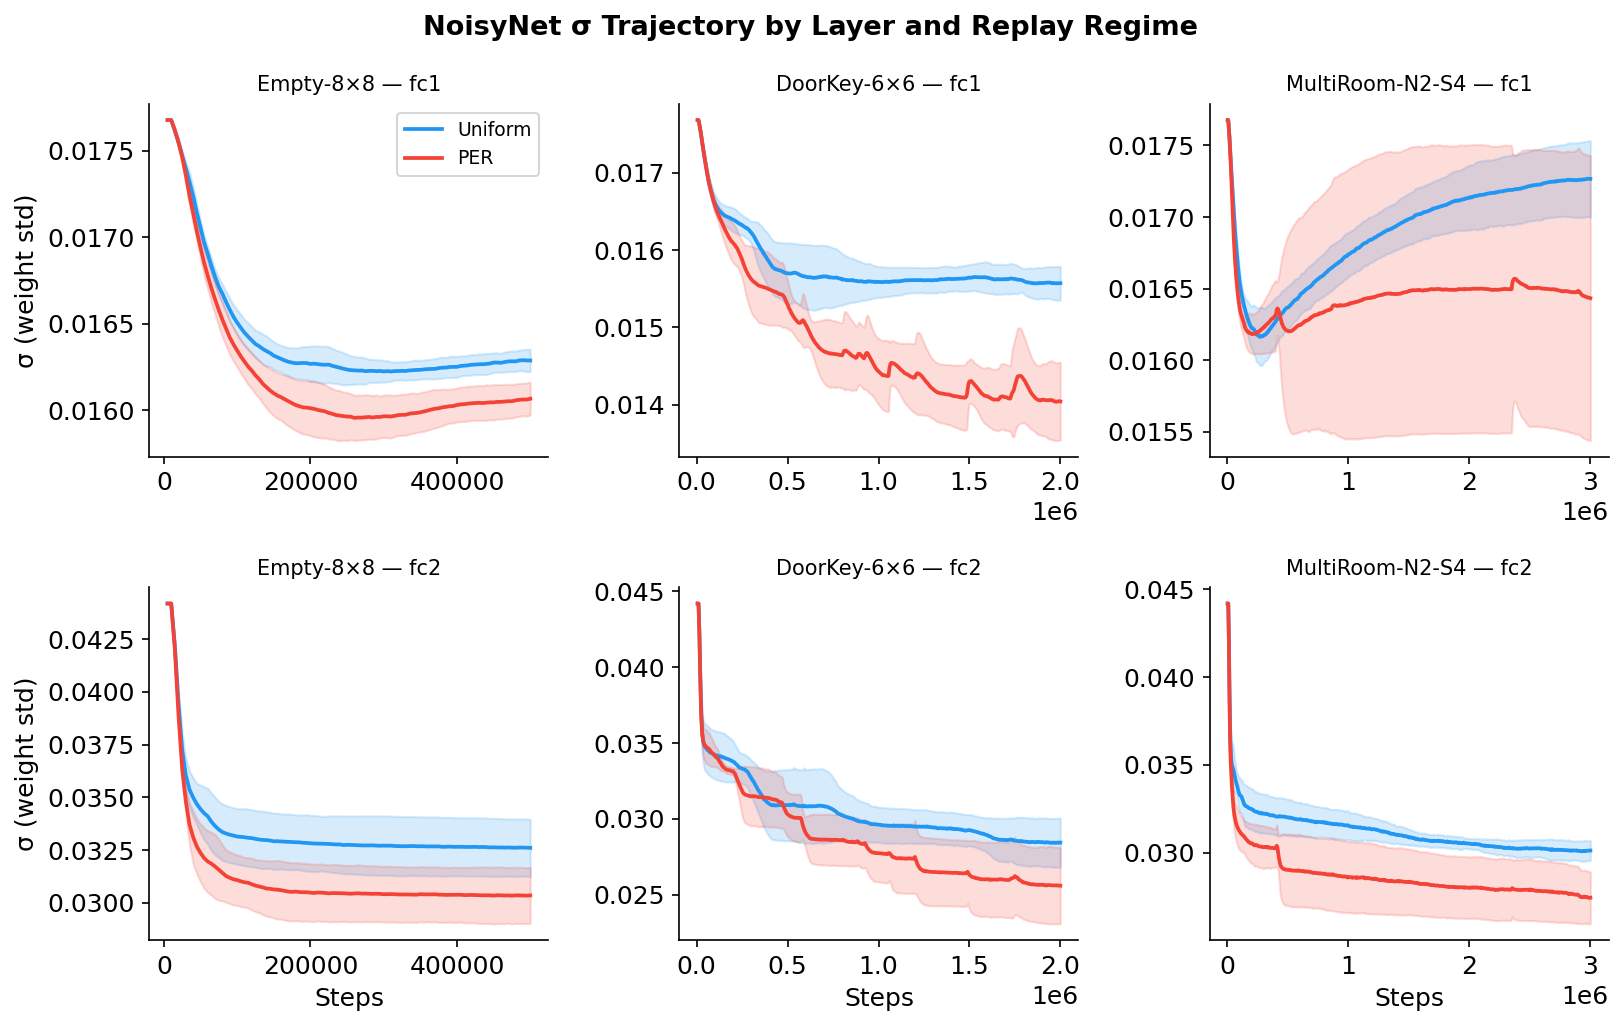
\includegraphics[width=\textwidth]{runs/plots_factorial/fig4_sigma_trajectory.png}
    \caption{NoisyNet $\sigma$ decay by layer and replay regime.}
    \label{fig:sigma}
  \end{subfigure}
  \hfill
  \begin{subfigure}[b]{0.45\textwidth}
    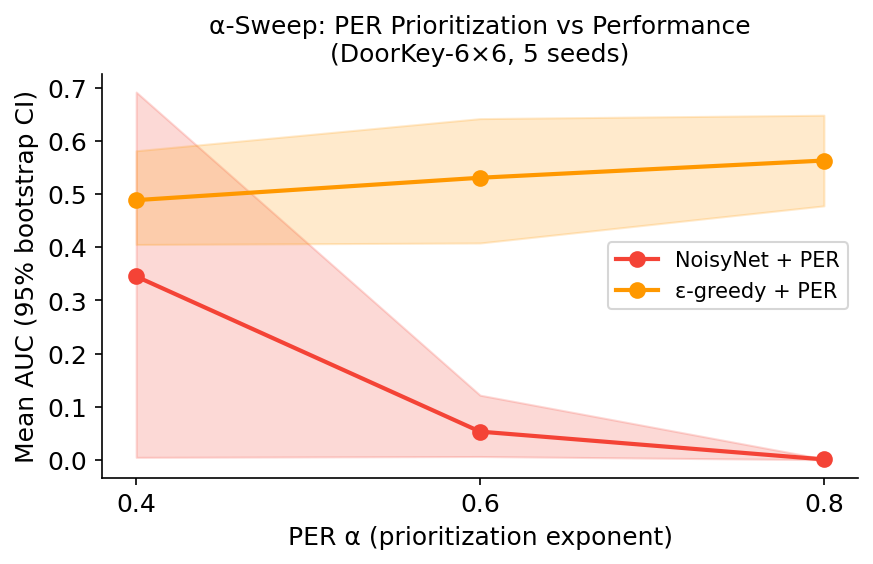
\includegraphics[width=\textwidth]{runs/plots_alpha_sweep/figA1_alpha_sweep_curves.png}
    \caption{$\alpha$-sweep: AUC vs.\ prioritization strength.}
    \label{fig:alpha}
  \end{subfigure}
  \caption{(a) PER accelerates $\sigma$ collapse relative to uniform replay,
           most severely in MultiRoom.
           (b) The two exploration regimes respond to $\alpha$ in
           \emph{opposite directions}: $\varepsilon$-greedy$+$PER improves
           monotonically; NoisyNet$+$PER collapses.}
  \label{fig:mech}
\end{figure}

\paragraph{$\sigma$ collapse.}
Figure~\ref{fig:sigma} shows the per-layer weight noise $\sigma$ over
training, split by replay regime (NoisyNet conditions only).
Under uniform replay, $\sigma$ decays gradually as the agent learns
a stable policy.
Under PER, $\sigma$ decays faster and reaches a lower floor---most
severely in MultiRoom, where PER drives $\sigma$ below $0.02$ before
the agent has encountered the sparse reward signal.
Once $\sigma$ is small, the network behaves near-deterministically and
cannot explore the key--door sequence.

The mechanism connects to Carrasco-Davis et al.~\cite{carrasco2025uper}
(UPER): PER treats TD error as a proxy for informativeness, but high
TD error can arise from weight noise rather than genuine surprise.
Early in training, when $\sigma$ is large, nearly every transition has
elevated stochastic TD error.
PER over-samples these transitions, effectively training the network to
regress away its own noise.
This is self-defeating: the exploration budget is spent suppressing the
exploration mechanism.

\paragraph{Bimodal failure in DoorKey.}
The bimodal outcome (3 fail / 2 partial success) reflects the race between
$\sigma$-collapse and reward discovery.
All five NoisyNet$+$PER seeds reach $\sigma \approx 0.022$--$0.025$ by
250k steps---indistinguishable across seeds.
Whether a seed succeeds depends entirely on whether the agent stumbled on
the key--door sequence \emph{before} $\sigma$ became too small to explore
further: a stochastic event that accounts for the bimodality.

% ─────────────────────────────────────────────────────────────────────────────
\section{$\alpha$-Sweep}
\label{sec:alpha}
% ─────────────────────────────────────────────────────────────────────────────

Figure~\ref{fig:alpha} and Table~\ref{tab:alpha} show AUC as a function of
prioritization strength $\alpha$ on DoorKey-6$\times$6.
The two regimes respond in \emph{opposite directions}:

\begin{table}[h]
\centering
\caption{AUC vs.\ $\alpha$ on DoorKey-6$\times$6 (mean, 95\% CI, 5 seeds).}
\label{tab:alpha}
\small
\begin{tabular}{lcccc}
\toprule
\textbf{Condition} & $\alpha=0.4$ & $\alpha=0.6$ & $\alpha=0.8$ \\
\midrule
NoisyNet$+$PER   & $0.345\;[0.005,\,0.692]$ & $0.054\;[0.007,\,0.122]$ & $0.001\;[0.001,\,0.002]$ \\
$\varepsilon$-greedy$+$PER & $0.489\;[0.404,\,0.581]$ & $0.531\;[0.408,\,0.642]$ & $0.563\;[0.478,\,0.648]$ \\
\bottomrule
\end{tabular}
\end{table}

For $\varepsilon$-greedy$+$PER, more aggressive prioritization is
monotonically beneficial, consistent with the standard PER finding on
deterministic exploration.
For NoisyNet$+$PER, more aggressive prioritization accelerates $\sigma$
collapse: at $\alpha=0.8$, NoisyNet$+$PER achieves essentially zero reward
across all five seeds.
At $\alpha=0.4$, performance partially recovers (mean AUC $0.345$), though
with high variance (std $0.416$)---the bimodal failure pattern persists even
at reduced prioritization.
This confirms that the interaction effect is not an artifact of the specific
$\alpha=0.6$ default: the two regimes have \emph{opposite} optimal $\alpha$,
and their performance curves diverge monotonically.

% ─────────────────────────────────────────────────────────────────────────────
\section{Discussion and Conclusion}
% ─────────────────────────────────────────────────────────────────────────────

We present the first controlled factorial study of the NoisyNet$\times$PER
interaction.
Across three environments and 80 total runs, we find:
\begin{enumerate}
\item PER reliably harms NoisyNet (negative interaction term in all
      environments, significant in two).
\item The mechanism is $\sigma$-collapse: PER over-samples high-noise
      transitions, training the network to suppress its own exploration before
      reward is discovered.
\item The interaction is monotone in $\alpha$: standard PER settings are
      actively harmful to NoisyNet, and the damage worsens with increasing
      prioritization strength.
\end{enumerate}

\paragraph{Practical implications.}
Practitioners combining NoisyNet with PER (as in Rainbow and its variants)
should be aware that the default $\alpha=0.6$ may suppress NoisyNet's
exploration.
Using a lower $\alpha$, or an exploration-aware prioritization scheme such as
UPER~\cite{carrasco2025uper}, may recover performance.

\paragraph{Limitations.}
Our study uses MiniGrid environments and a small CNN backbone; results on
Atari-scale tasks may differ.
Five seeds is adequate for two significant environments but leaves DoorKey
inconclusive.
The $\alpha$-sweep is limited to $\{0.4, 0.6, 0.8\}$; finer resolution and
lower $\alpha$ values (e.g., $0.1$--$0.3$) may clarify the recovery regime.

\paragraph{Future work.}
The natural next step is an exploration-aware priority function that discounts
TD error by the current $\sigma$ level of the relevant weights, preventing PER
from treating exploration noise as informative signal.
We leave this as a design challenge motivated by the present results.

% ─────────────────────────────────────────────────────────────────────────────

\bibliographystyle{plainnat}
\bibliography{references}

\end{document}
